\documentclass[11pt,a4paper,twocolumn]{article}

% === Core Packages ===
\usepackage[margin=2cm]{geometry}
\usepackage[utf8]{inputenc}
\usepackage[T1]{fontenc}
\usepackage{times}
\usepackage{amsmath,amssymb}
\usepackage{graphicx}
\usepackage{booktabs}
\usepackage{float}
\usepackage{enumitem}
\usepackage{tikz}
\usepackage{pgfplots}
\pgfplotsset{compat=1.18}
\usetikzlibrary{arrows.meta,shapes.geometric,positioning,calc,decorations.markings,fit,backgrounds}

% === Citation (IEEE style) ===
\usepackage[numbers,sort&compress]{natbib}
\bibliographystyle{IEEEtranN}

% === Hyperref ===
\usepackage[hidelinks]{hyperref}
\usepackage{xurl}

% === Settings ===
\setlength{\parindent}{1em}
\setlength{\parskip}{0.3em}

% === PDF metadata ===
\hypersetup{
  pdftitle={Decentraliseret Omdømmenetværk: En Ramme for Naturlig Samfundsorganisering},
  pdfauthor={Pavel Kudrna},
  pdfsubject={Personix — a decentralized reputation network},
  pdfkeywords={Personix, decentralized reputation, reputation social network,
    decentralized identifiers, DID, meritocracy, censorship resistance},
}

% === Title ===
\title{\textbf{Decentraliseret Omdømmenetværk:\\En Ramme for Naturlig Samfundsorganisering}}
\author{Pavel Kudrna\\Personix Project --- \url{https://personix.org}\\Prague, Czechia\\Draft v1 --- March 2026}
\date{}

\begin{document}
\maketitle

% ============================================================
% ABSTRACT
% ============================================================
\begin{abstract}
Retfærdighedssansen---overbevisningen om, at uret bliver gjort godt igen, og at fortjeneste bliver belønnet---er samfundets stærkeste sammenbindende kraft. Når centraliserede forvaltningsinstitutioner ikke kan levere denne følelse, fordi omkostningen ved at håndhæve en ret overstiger værdien af selve retten, eroderer den sociale sammenhængskraft. Nuværende institutionelle strukturer formår ikke at løse en betydelig klasse af tvister på systematisk samme måde, som central planlægning fejler i at allokere ressourcer: gennem informationsasymmetri, manglende feedbacksløjfer og afkobling af beslutningstagere fra konsekvenserne af deres beslutninger. Denne artikel præsenterer et Omdømmesocialt Netværk (RSN): et decentraliseret, ubestikkeligt, censurbestandigt kommunikationslag bygget på Decentraliserede Identifikatorer (DID'er), der gør det muligt for pseudonyme deltagere at publicere, verificere og forbruge omdømmeinformation om adfærd i den virkelige verden. Kernemekanismen hviler på tre designprincipper: (1)~en asymmetrisk omkostningsstruktur, hvor det er billigt at læse omdømmedata, men at skrive kræver verificerbar indsats; (2)~en ikke-deterministisk protokol for udvælgelse af verifikatorer baseret på konsistent hashing, der prissætter radikale påstande gennem eskalerende iterationsomkostninger; og (3)~en markedsdrevet model for omdømmeautoritet, hvor private verifikatorer sætter deres akkumulerede omdømme på spil på nøjagtigheden af de påstande, de går god for. Den resulterende arkitektur frembringer emergent meritokrati uden central koordinering og muliggør en gradvis, reversibel migrationsvej fra eksisterende statsadministrerede systemer.
\end{abstract}

% ============================================================
% 1. INTRODUCTION
% ============================================================
\section{Introduktion}

\subsection{Problemet med Centraliseret Tillid}

Moderne forvaltning hviler på en grundlæggende antagelse: at centraliserede institutioner kan mægle tillid mellem fremmede i stor skala. Domstole afgør tvister. Registre certificerer ejerskab. Regulerende organer håndhæver standarder. Disse institutioner blev udformet i en tid, hvor information var knap, kommunikation var langsom, og delegering af myndighed til et centralt organ var den eneste gennemførlige koordineringsmekanisme. Centraliseret forvaltning fejler imidlertid af de samme strukturelle årsager som central planlægning: informationsasymmetri, manglende feedbacksløjfer og afkobling af beslutningstagere fra konsekvenserne af deres beslutninger.

Antagelsen fejler for eksempel, når omkostningen ved institutionel mægling overstiger tvistens værdi. Betragt en lejer, der opdager, at deres lejede lejlighed mangler et lovpligtigt elsikkerhedscertifikat---en tilstand, der udgør en umiddelbar livsfare. Lejerens juridiske ret til at træde ud af kontrakten er utvetydig. Alligevel overstiger omkostningen ved at håndhæve denne ret gennem retssystemet den pengemæssige værdi af depositummet og de skyldige erstatninger, selv medregnet potentiel lovbestemt kompensation~\cite{czcourtfees}. Den rationelle reaktion er at absorbere tabet og træde ud.

Dette er ikke et patologisk grænsetilfælde. Det er standardoplevelsen for en betydelig klasse af tvister, hvor skaden er reel, men de pengemæssige indsatser falder under den tærskel, hvor institutionel håndhævelse bliver økonomisk rationel. Resultatet er et system, der strukturelt begunstiger onde aktører: dem, der skader andre i mængder under denne tærskel, kan handle ustraffet, fordi omkostningen ved at søge retfærdighed falder på den skadelidte part.

Ovenstående eksempel er hentet fra forfatterens juridiske miljø---det tjekkiske civilretlige system. I andre retstraditioner---præcedensbaseret common law, sædvaneret, blandede systemer---fejler retfærdigheden på forskellige måder og i forskellig grad, afhængigt af jurisdiktionens kulturelle og procesmæssige særtræk. Læsere vil sandsynligvis genkende tilsvarende eksempler fra deres egen kontekst. Hvad der er strukturelt universelt, er mønsteret: tvister, hvis værdi falder under tærsklen for økonomisk rationel håndhævelse, ender med, at tabet absorberes af den skadelidte part. RSN lover ikke perfekt retfærdighed---det reducerer blot den strukturelle fordel, som onde aktører nyder, når institutionel håndhævelse er uøkonomisk.

\subsection{Hvorfor Eksisterende Løsninger Kommer til Kort}

\textbf{Rammer for Decentraliseret Identitet (DID)}~\cite{did2022} tilvejebringer kryptografiske mekanismer til selvsuveræn identitetshåndtering, men fokuserer primært på identitetsverifikation uden at adressere det bredere spørgsmål om adfærdsmæssigt omdømme.

\textbf{Soulbound-tokens (SBT'er)}~\cite{weyl2022} indfanger den indsigt, at omdømme er ikke-overførbart, men er afhængige af blockchain-infrastruktur med skalerbarhedsbegrænsninger og adresserer ikke de økonomiske incitamenter, der styrer indførsel af information. Beslægtede koncepter som meritt-tokens (f.eks. Liberland) deler en lignende filosofi, men forbliver bundet til specifikke jurisdiktionelle rammer.

\textbf{Decentraliserede Autonome Organisationer (DAO'er)}~\cite{buterin2014} implementerer forvaltning gennem smart contracts, men reproducerer plutokratiske dynamikker, hvor indflydelse er proportional med kapital. Kvadratisk afstemning~\cite{buterin2019} afbøder dette delvist, men begrænser praktisk udbredelse. DAO'er står også over for det grundlæggende \emph{orakelproblem}: smart contracts kan ikke pålideligt verificere tilstande i den virkelige verden uden en betroet ekstern kilde, og dette problem har ingen generel løsning inden for blockchain-arkitektur.

Intet eksisterende system kombinerer decentralisering, censurbestandighed, pseudonymitet, verificerbare adgangsomkostninger og emergent konsensus.

\subsection{Bidrag}

Denne artikel yder følgende bidrag:
\begin{enumerate}[nosep]
\item Definition af \textbf{Omdømmesocialt Netværk (RSN)}, en decentraliseret protokol, der udvider DID-rammen til at understøtte bilateral omdømmeudveksling.
\item En \textbf{ikke-deterministisk protokol for udvælgelse af verifikatorer} baseret på konsistent hashing~\cite{karger1997}.
\item \textbf{Princippet om Dyr Radikalisme}, der prissætter påstande efter deres afstand fra netværkskonsensus gennem tre kumulerende omkostningskanaler.
\item En \textbf{model for Omdømmeautoritet} med asymmetriske incitamenter, hvor falsk godkendelse koster katastrofalt mere end legitime gebyrer.
\item En \textbf{gradvis migrationsvej} gennem parallel finanspolitisk infrastruktur.
\end{enumerate}

% ============================================================
% 2. DESIGN PRINCIPLES
% ============================================================
\section{Designprincipper}

RSN-arkitekturen er begrænset af fem ikke-forhandlelige designprincipper.

\textbf{Kontinuitet og Udvikling.} Systemet sameksisterer med eksisterende institutioner i en overgangsperiode af ubestemt længde. Overgangen skal være reversibel på ethvert stadie.

\textbf{Frivillighed og Ansvar.} Deltagelse er frivillig, men frivillighed er koblet til ansvar: en deltager, der påtager sig kontrol over en institutionel funktion, påtager sig samtidig de medfølgende forpligtelser.

\textbf{Mangfoldighed og Kulturel Neutralitet.} Konsensus opstår ud fra bilaterale interaktioner, ikke ud fra forudindstillede regler pålagt af systemdesignere.

\textbf{Modstandsdygtighed og Censurbestandighed.} Omkostningen ved at censurere netværket skal overstige omkostningen ved at tolerere det. Kun fuld totalitarisme---til ruinerende politisk og økonomisk pris---kan undertrykke systemet.

\textbf{Konsensus og Håndhævelse.} Systemet indarbejder menneskelige tilbøjeligheder til smålighed, ondskabsfuldhed og gengældende tilfredsstillelse som bærende træk. Forseelser er ikke forbudte; de prissættes.

% ============================================================
% 3. SYSTEM OVERVIEW
% ============================================================
\section{Systemoversigt}

\subsection{Omdømmesocialt Netværk}

RSN er et decentraliseret peer-to-peer-kommunikationslag, hvor deltagere udveksler verificerbar information om adfærd i den virkelige verden. Dets definerende egenskaber er: decentraliseret og ucensurerbar infrastruktur; pseudonym deltagelse gennem DID'er; asymmetrisk omkostningsstruktur (læsning er billig, skrivning er dyr); kryptografisk verificerbarhed; og \textbf{standardunderstøttelse}---maskinlæsbare formater for information, der udbredes gennem netværket, for tjenester tilbudt af autoriteter (sammensætning af påstande, godkendelse, vidnetjeneste) og for policy-formatet, herunder regler for evaluering af modpartens omdømme og vurdering af risikoen for policy-uoverensstemmelse (mellem erklæret og faktisk adfærd).

\subsection{Arkitektoniske Komponenter}

RSN består af fire primære komponenter (Fig.~\ref{fig:architecture}):
\begin{enumerate}[nosep]
\item \textbf{DID-lag.} Deltageridentiteter med erklærede regler, omdømmemetadata og netværksrouting.
\item \textbf{Påstandsprotokol.} Struktureret format til publicering af udsagn om hændelser i den virkelige verden.
\item \textbf{Verifikationsnetværk.} Decentraliseret protokol til tildeling af verifikatorer ved hjælp af konsistent hashing.
\item \textbf{Omdømmeaggregeringslag.} Tjenester, der producerer menneskelæsbare omdømmesammendrag.
\end{enumerate}

\begin{figure}[ht]
\centering
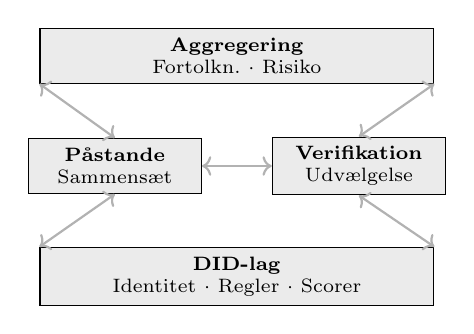
\begin{tikzpicture}[
    layer/.style={draw, minimum height=0.7cm, align=center, font=\scriptsize, fill=black!8},
    arr/.style={<->, thick, gray!60}
]
\node[layer, minimum width=5cm] (agg) at (0,2.8) {\textbf{Aggregering}\\Fortolkn.\ $\cdot$ Risiko};
\node[layer, minimum width=2.2cm] (claim) at (-1.55,1.4) {\textbf{Påstande}\\Sammensæt};
\node[layer, minimum width=2.2cm] (verif) at (1.55,1.4) {\textbf{Verifikation}\\Udvælgelse};
\node[layer, minimum width=5cm] (did) at (0,0) {\textbf{DID-lag}\\Identitet $\cdot$ Regler $\cdot$ Scorer};

\draw[arr] (agg.south west) -- (claim.north);
\draw[arr] (agg.south east) -- (verif.north);
\draw[arr] (claim.east) -- (verif.west);
\draw[arr] (claim.south) -- (did.north west);
\draw[arr] (verif.south) -- (did.north east);
\end{tikzpicture}
\caption{RSN's firelagsarkitektur.}
\label{fig:architecture}
\end{figure}

\subsection{Deltagerroller}

En verifikationstransaktion involverer op til seks særskilte DID-roller (Fig.~\ref{fig:roles}): \textbf{Udsteder} ($DID_I$, opretter og indsender påstanden), \textbf{Subjekt} ($DID_S$, den DID som påstanden handler om---kan være sammenfaldende med Udsteder), \textbf{Autoritet} ($DID_A$, godkender påstanden mod et gebyr; kan også tilbyde vidnetjenester---\emph{valgfri}), \textbf{Vidne} ($DID_{W_{1..n}}$, inkognito overvåger af verifikatorens hæderlighed via udfordringskoder---\emph{valgfri}), \textbf{Verifikator} ($DID_V$, algoritmisk udvalgt til at publicere påstanden) og \textbf{RSN} (netværket hvor verificerede påstande publiceres). Enhver rolle kan delegeres til en anden DID (Afsnit~7.4). En Autoritet samler almindeligvis godkendelse med vidnetjenester, men de to funktioner er logisk uafhængige.

\begin{figure}[ht]
\centering
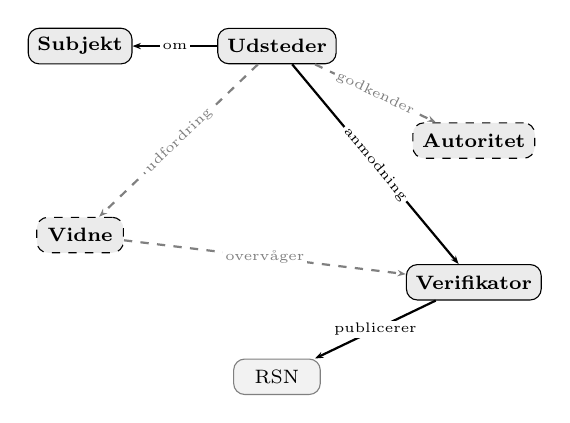
\begin{tikzpicture}[
    role/.style={draw, rounded corners, minimum width=1.1cm, minimum height=0.45cm, align=center, font=\scriptsize, fill=black!8},
    opt/.style={draw, rounded corners, minimum width=1.1cm, minimum height=0.45cm, align=center, font=\scriptsize, fill=black!8, dashed},
    arr/.style={-{Stealth[length=3pt]}, thick},
    oarr/.style={-{Stealth[length=3pt]}, thick, dashed, gray},
    lbl/.style={font=\tiny, fill=white, inner sep=1pt}
]
\node[role] (I) at (0,2.4) {\textbf{Udsteder}};
\node[role] (S) at (-2.5,2.4) {\textbf{Subjekt}};
\node[opt] (A) at (2.5,1.2) {\textbf{Autoritet}};
\node[opt] (W) at (-2.5,0) {\textbf{Vidne}};
\node[role] (V) at (2.5,-0.6) {\textbf{Verifikator}};
\node[role, fill=black!5, draw=gray] (N) at (0,-1.8) {RSN};

\draw[arr] (I) -- node[lbl] {om} (S);
\draw[oarr] (I) -- node[lbl,sloped] {godkender} (A);
\draw[oarr] (I) -- node[lbl,sloped] {udfordring} (W);
\draw[arr] (I) -- node[lbl,sloped] {anmodning} (V);
\draw[oarr] (W) -- node[lbl] {overvåger} (V);
\draw[arr] (V) -- node[lbl] {publicerer} (N);
\end{tikzpicture}
\caption{DID-roller i en verifikationstransaktion. Stiplet = valgfri (Autoritet, Vidne).}
\label{fig:roles}
\end{figure}

\subsection{Ubestikkelighed: Fire Kræfter}

RSN's ubestikkelighed udspringer ikke af en enkelt mekanisme, men af fire samtidige kræfter. Ingen er tilstrækkelig i sig selv; kun deres kombination gør et forsøg på korruption økonomisk irrationelt.

\textbf{Uforudsigeligt mål.} Verifikatoren for hver påstand udvælges ikke-deterministisk gennem konsistent hashing (Afsnit~5.3). En angriber kan ikke på forhånd udpege en bestemt verifikator til bestikkelse, fordi verifikatorens identitet er en funktion af påstandens indhold og tidligere iterationer, ikke af udstederens valg.

\textbf{Omdømmets løftestang---langsomt op, hurtigt ned.} Omdømme kan kun opnås gradvist, gennem vedvarende konsistent adfærd. Det kan imidlertid tabes katastrofalt i en enkelt bedragerisk godkendelse (Afsnit~6.2). Denne asymmetri betyder, at års akkumuleret omdømme kan ødelægges af én uhæderlig godkendelse; den optimale strategi forbliver at afvise mistænkelige påstande.

\textbf{Offentligt løfte.} Enhver DID-Indehaver erklærer offentligt sin policy---et maskinlæsbart sæt regler, som de forpligter sig til at følge. Afvigelse mellem erklæringen og den faktiske adfærd er detekterbar og prissættes som en omdømmemæssig forseelse, der er alvorligere end den underliggende overtrædelse (Afsnit~7.3). Hykleri er derfor dyrere end direkte uhæderlighed.

\textbf{Mesh-netværkets asymmetri i angrebsomkostninger.} Omkostningen ved at censurere eller destabilisere netværket vokser ikke-lineært med netværkets størrelse og tæthed, mens omkostningen ved at tolerere det forbliver konstant. For at censur skal betale sig, ville en centraliseret aktør skulle anvende den på tværs af hele netværket---hvilket kræver foranstaltninger, der er uforholdsmæssige i forhold til enhver tænkelig fordel (Afsnit~10).

% ============================================================
% 4. DECENTRALIZED IDENTITY MODEL
% ============================================================
\section{Model for Decentraliseret Identitet}

\subsection{DID med Særlige Egenskaber}

RSN udvider W3C DID Core-specifikationen~\cite{did2022} med: \textbf{Erklærede Regler} (maskinlæsbare adfærdsforpligtelser), \textbf{Omdømmemetadata} (aggregeret adfærdsscore) og \textbf{Netværksrouting} (foranderlig onion-gateway adskilt fra den stabile ringposition).

\subsection{Påstandens Livscyklus}

En Påstand forløber gennem seks stadier (Fig.~\ref{fig:lifecycle}): sammensætning, valgfri godkendelse af autoritet, udvælgelse af verifikator via konsistent hashing, verifikationsbeslutning (accepter eller afvis med iteration), publicering og omdømmeopdatering for alle parter.

\begin{figure}[ht]
\centering
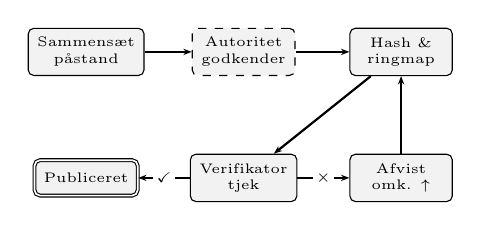
\begin{tikzpicture}[
    stp/.style={draw, rounded corners=2pt, minimum width=1.3cm, minimum height=0.45cm, align=center, font=\tiny, fill=black!5},
    arr/.style={-{Stealth[length=3pt]}, thick},
    lbl/.style={font=\tiny, fill=white, inner sep=1pt}
]
\node[stp] (comp) at (0,0) {Sammensæt\\påstand};
\node[stp, dashed] (auth) at (2.0,0) {Autoritet\\godkender};
\node[stp] (hash) at (4.0,0) {Hash \&\\ringmap};
\node[stp] (ver) at (2.0,-1.6) {Verifikator\\tjek};
\node[stp, double] (pub) at (0,-1.6) {Publiceret};
\node[stp] (rej) at (4.0,-1.6) {Afvist\\omk. $\uparrow$};

\draw[arr] (comp) -- (auth);
\draw[arr] (auth) -- (hash);
\draw[arr] (hash) -- (ver);
\draw[arr] (ver) -- node[lbl] {\checkmark} (pub);
\draw[arr] (ver) -- node[lbl] {$\times$} (rej);
\draw[arr] (rej) -- ++(0,0.8) -| (hash);
\end{tikzpicture}
\caption{Påstandens livscyklus med iterationssløjfe.}
\label{fig:lifecycle}
\end{figure}

\subsection{Forhold til W3C DID Core}

RSN's identitetsmodel er en ægte overmængde af W3C DID Core-specifikationen~\cite{did2022}. Alle RSN-DID'er er gyldige W3C-DID'er. De RSN-specifikke udvidelser er kodet som DID-dokumentegenskaber defineret i en dedikeret DID-metodespecifikation, kompatibel med eksisterende infrastruktur såsom ION~\cite{buchner2021} og Ceramic~\cite{ceramic2023}.

% ============================================================
% 5. VERIFICATION AND PROPAGATION
% ============================================================
\section{Verifikation og Udbredelse af Information}

\subsection{Omkostningen ved Indførsel af Information}

RSN's økonomiske kerneprincip er asymmetrien mellem læsning og skrivning. At læse omdømmedata nærmer sig nul i marginalomkostning for deltagere, der er en del af DID-netværket og har adgang svarende til deres omdømme---nytilkomne må gradvist optjene bredere adgang (se anti-snylteri). Skrivning---forstået som den varige materialisering af omdømme ind i netværket, ikke som en engangsteknisk handling---kræver verificerbar kumulativ investering på tværs af tre dimensioner: \textbf{tid} (leveår brugt på konsistent adfærd, opfyldte forpligtelser og plejede relationer), \textbf{energi} (indsats investeret i hæderlig handel, omsorg for partnerskaber og langsigtet troværdighed) og \textbf{penge} (investering i ens eget navn---faglig udvikling, kvaliteten af ens arbejde, genoprettelse for forvoldte skader). Omdømme kan ikke købes øjeblikkeligt---det er resultatet af livslang akkumulering, som systemet blot gør synligt og overførbart på tværs af kontekster. Protokollens engangstekniske omkostninger (kryptografiske signaturer, verifikatorgebyrer) er ubetydelige sammenlignet med denne underliggende investering.

\subsection{Social Graf og Kontaktdybde}

RSN er grundlæggende et socialt netværk: hver DID tilføjer kontakter (andre DID'er), der tillader forbindelsen. Disse kontakter har deres egne kontakter, og så videre. Den algoritmiske søgning efter verifikator opererer inden for en konfigurerbar dybde $h$ af sammenkædede kontakter (f.eks. $h=3$: ens direkte kontakter, deres kontakter og kontakters kontakter). Denne arkitektur kræver ikke en enkelt global blockchain---den favoriserer naturligt fremkomsten af fællesskaber/klynger med overlap til andre fællesskaber. Enhver DID-deltager skal have en publiceret \textbf{policy}---et maskinlæsbart sæt regler, der styrer, hvordan indkommende anmodninger evalueres. Policy-overtrædelser registreres i netværket som negative artefakter.

\subsection{Algoritmisk Udvælgelse af Verifikator}

Verifikationsprotokollen anvender konsistent hashing~\cite{karger1997} (Fig.~\ref{fig:verifier}). Verifikation er en betalt tjeneste: verifikatorer arbejder mod et gebyr, hvilket skaber et marked, hvor konkurrence driver prissætning, hastighed og pålidelighed.

\textbf{Trin 1.} Påstandsdokumentet sammenkædes med den foregående iterations hash-resultat (eller $\varnothing$ ved første iteration) og hashes:
\begin{equation}
\text{pos} = f_h(\text{claim} \| \text{prev\_hash})
\label{eq:hash}
\end{equation}

Algoritmen skal inkludere den \emph{komplette sti} af alle tidligere anmodninger og svar---ikke blot en hash af den foregående iteration. Hver verifikators fulde svar (accept, afvisning, tilbudt pris, begrundelse) føjes til det voksende dokument, verificerbart gennem kryptografiske signaturer ved hvert trin.

\textbf{Trin 2.} Hashen kortlægges til $N$ positioner på den konsistente hash-ring, jævnt fordelt (f.eks. for $N=4$: $+0^{\circ}, +90^{\circ}, +180^{\circ}, +270^{\circ}$). Fra hver position udvælger en søgning med uret den nærmeste DID som verifikatorkandidat (Fig.~\ref{fig:multipoint}). $N$ er en variabel parameter, der kan afhænge af procentdelen af aktuelt aktive DID'er, tidspunktet på dagen eller netværkets historiske svartid.

\textbf{Trin 3.} Verifikatoren accepterer (publicerer, sætter omdømme på spil) eller afviser (vender tilbage til Trin~1 med afvisningens hash). Når en node ikke svarer på trods af at erklære online-status, skal den næste anmodning inkludere alle svar fra alle $N$ tidligere verifikatorkandidater.

\textbf{Anti-snylteri.} Mål-DID'er kan fastsætte gebyrer eller adgangsbegrænsninger for forespørgsler fra nye DID'er med lidt omdømme. Denne gradvise mekanisme (ikke binær) tvinger nytilkomne til at opbygge omdømme gennem ægte aktivitet, før de frit forbruger andres data.

\begin{figure}[ht]
\centering
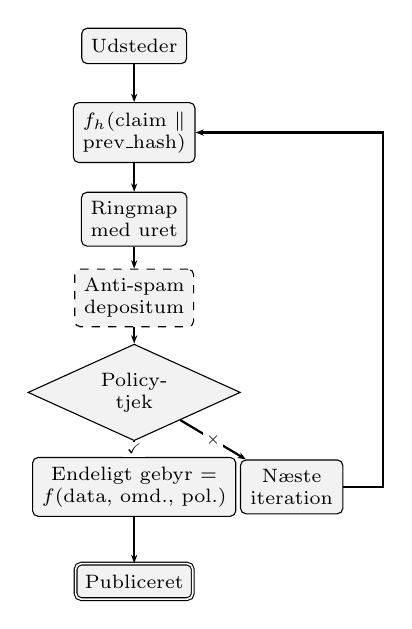
\begin{tikzpicture}[
    box/.style={draw, rounded corners=2pt, minimum width=1.3cm, minimum height=0.45cm, align=center, font=\scriptsize, fill=black!5},
    dec/.style={draw, diamond, aspect=2.2, minimum width=0.9cm, align=center, font=\scriptsize, fill=black!5},
    arr/.style={-{Stealth[length=3pt]}, thick},
    lbl/.style={font=\tiny, fill=white, inner sep=1pt}
]
\node[box] (iss) at (0,0) {Udsteder};
\node[box] (hash) at (0,-1.1) {$f_h$(claim $\|$\\prev\_hash)};
\node[box] (ring) at (0,-2.2) {Ringmap\\med uret};
\node[box, dashed] (spam) at (0,-3.2) {Anti-spam\\depositum};
\node[dec] (check) at (0,-4.4) {Policy-\\tjek};
\node[box] (rej) at (2,-5.6) {Næste\\iteration};
\node[box] (fee) at (0,-5.6) {Endeligt gebyr =\\$f$(data, omd., pol.)};
\node[box, double] (pub) at (0,-6.8) {Publiceret};

\draw[arr] (iss) -- (hash);
\draw[arr] (hash) -- (ring);
\draw[arr] (ring) -- (spam);
\draw[arr] (spam) -- (check);
\draw[arr] (check) -- node[lbl] {$\times$} (rej);
\draw[arr] (check) -- node[lbl] {\checkmark} (fee);
\draw[arr] (fee) -- (pub);
\draw[arr] (rej.east) -- ++(0.5,0) |- (hash.east);
\end{tikzpicture}
\caption{Protokol for udvælgelse af verifikator. Anti-spam-depositum er valgfrit og kan være tilbagebetaleligt. Det endelige gebyr betales kun ved accept.}
\label{fig:verifier}
\end{figure}

Hver afvisning føjer verifikatorens fulde svar (herunder begrundelser og betingelser) til påstandsdokumentet og udvider dets indhold. Fra det udvidede dokument beregnes en ny hash ikke-deterministisk, som kortlægges til en anden ringposition og udvælger en anden verifikator. Dokumentation af den fulde sti er obligatorisk---udstederen kan ikke forudsige eller påvirke den næste verifikator. Hvis en verifikator ignorerer en anmodning på trods af en kompatibel erklæret policy, registrerer vidner (hvis til stede) dette, og udstederen kan vedhæfte vidneudsagn ved endelig publicering.

\begin{figure}[ht]
\centering
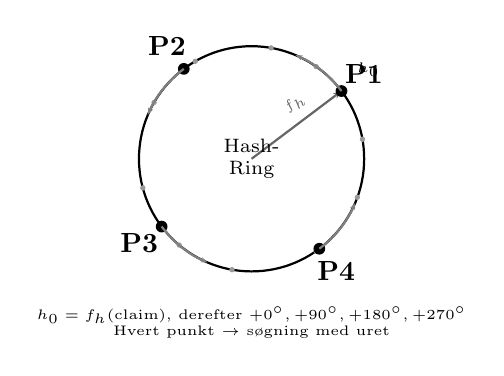
\begin{tikzpicture}[scale=0.65]
% Ring
\draw[thick] (0,0) circle (2.2cm);
% DID nodes on ring
\foreach \a in {10,55,80,120,150,195,230,260,305,340} {
  \fill[black!40] (\a:2.2) circle (1.5pt);
}
% Hash offset arrow pointing to initial position
\draw[-{Stealth[length=3pt]}, thick, black!60] (0,0) -- node[font=\tiny,above,sloped,pos=0.6] {$f_h$} (37:2.2);
\fill[black] (37:2.2) circle (2pt);
\node[font=\tiny,anchor=south west] at (37:2.35) {$h_0$};
% N=4 points offset from h0 by +0, +90, +180, +270
\foreach \offset/\l in {0/P1,90/P2,180/P3,270/P4} {
  \pgfmathsetmacro{\ang}{37+\offset}
  \node[fill=black, circle, inner sep=1.5pt] (p\offset) at (\ang:2.2) {};
  \node[font=\tiny,font=\bfseries] at (\ang:2.75) {\l};
  % clockwise search arc
  \draw[-{Stealth[length=2.5pt]}, thick, gray] (\ang:2.2) arc (\ang:\ang+30:2.2);
}
\node[font=\scriptsize, align=center] at (0,0) {Hash-\\Ring};
\node[font=\tiny, align=center] at (0,-3.2) {$h_0 = f_h(\text{claim})$, derefter $+0^{\circ},+90^{\circ},+180^{\circ},+270^{\circ}$\\Hvert punkt $\rightarrow$ søgning med uret};
\end{tikzpicture}
\caption{Multipunktsudvælgelse ($N{=}4$). Hash $h_0$ sætter forskydningen; 4 punkter jævnt fordelt fra $h_0$.}
\label{fig:multipoint}
\end{figure}

\subsection{Vidneprotokol}

\textbf{Vidne}-rollen tilvejebringer inkognito ansvarlighed for verifikatorens hæderlighed gennem en kryptografisk udfordringskode-protokol:

\textbf{Trin W1.} Anmoderen signerer verifikationsanmodningen og sender den til $N_w$ vidner---kontakter fra anmoderens sociale netværk eller specialiserede udbydere af vidnetjenester, der arbejder mod et gebyr.

\textbf{Trin W2.} Hvert vidne $w_i$ signerer hele den signerede anmodning, beholder den oprindelige signatur $\sigma_i$ og beregner en udfordringskode $c_i = h(\sigma_i)$. Udfordringskoden føjes til anmodningen.

\textbf{Trin W3.} Anmodningen, der nu bærer $N_w$ udfordringskoder, sendes til verifikatoren. Verifikatoren observerer koderne, men \emph{kan ikke afgøre}, hvem vidnerne er, eller hvorvidt koderne svarer til reelle signaturer.

\textbf{Trin W4 (hæderlig verifikator).} Hvis verifikatoren svarer i overensstemmelse med sin erklærede policy, forbliver udfordringskoderne uigennemsigtige. Vidner afsløres aldrig. Ingen yderligere data publiceres.

\textbf{Trin W5 (policy-overtrædelse).} Hvis verifikatoren overtræder sin policy (ignorerer anmodningen, svarer inkonsekvent), er anmoderen i besiddelse af vidnernes oprindelige signaturer $\sigma_i$. Disse kan publiceres som ledsagedata: enhver kan verificere $c_i = h(\sigma_i)$, hvilket beviser, at vidnet var til stede. Anmoderen kan publicere uafhængigt---verifikatoren har allerede signeret udfordringskoderne i sit svar.

\textbf{Bluff-egenskaben.} Anmoderen kan erstatte nogle eller alle udfordringskoder med tilfældige værdier. Verifikatoren kan ikke skelne ægte koder (understøttet af autoriteter med højt omdømme) fra støj. Denne \emph{usikkerhed} er håndhævelsesmekanismen: enhver anmodning bærer risikoen for, at en respekteret autoritet holder øje inkognito. Omkostningen ved at opretholde dette pres er tæt på nul (generering af tilfældige tal), mens den potentielle omkostning ved uhæderlighed for verifikatoren er katastrofal. Hæderlig adfærd tilskyndes selv i fravær af faktiske vidner.

\textbf{Autoritet som vidne.} En Autoritet, der godkender en påstand, kan samle vidnetjenester: ``Jeg godkender din påstand og fungerer som inkognito vidne under verifikationen.'' Dette er en naturlig forretningsmodel---Autoriteten har allerede konteksten. De to roller er dog logisk uafhængige.

\subsection{Princippet om Dyr Radikalisme}

Tre omkostningskanaler kumuleres samtidigt (Fig.~\ref{fig:radicalism}):

\textbf{Kanal 1: Iterationsomkostning.} Hver afvisning fremtvinger en ny iteration, der forbruger tid og ressourcer. Lineær vækst.

\textbf{Kanal 2: Dokumentopsvulmning.} Hver iteration føjer verifikatorens fulde svar til påstandsdokumentet. Væksten er lineær, men med en basisforskydning: den indledende payload (påstandsindhold, autoritetsgodkendelse, kryptografiske signaturer) har allerede en ikke-triviel størrelse $B_0$. Samlet størrelse efter $k$ iterationer: $S(k) = B_0 + k \cdot \Delta$, hvor $\Delta$ er den gennemsnitlige svarstørrelse.

\textbf{Kanal 3: Verifikatorens Risikopræmie.} Risiko er subjektiv. Verifikatoren vurderer, om den anmodende DID's erklærede policyer er i konflikt med verifikatorens egne kommercielle, sociale eller politiske interesser. Præmien kan eskalere eksponentielt med den opfattede afstand fra verifikatorens ``ideal'': $P(d) = \alpha \cdot e^{\beta d}$, hvor $d$ er verifikatorens subjektive afstandsmål. Ud over en personlig no-go-grænse kan verifikatoren afvise fuldstændigt.

\begin{figure}[ht]
\centering
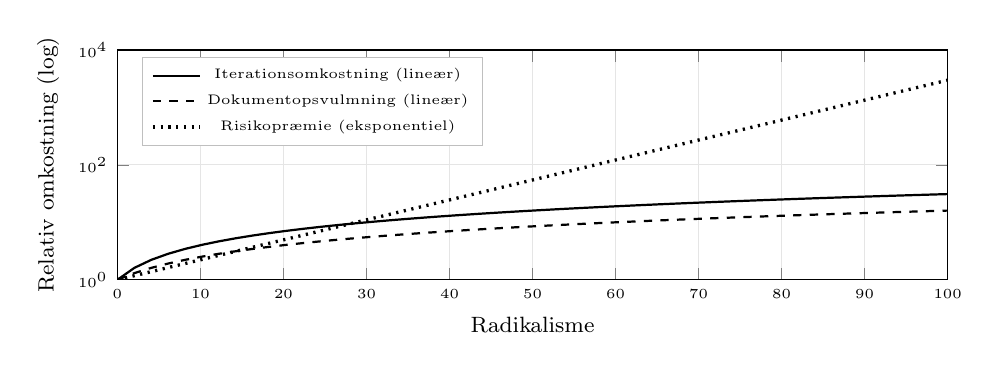
\begin{tikzpicture}
\begin{axis}[
    width=\columnwidth,
    height=4.5cm,
    xlabel={\footnotesize Radikalisme},
    ylabel={\footnotesize Relativ omkostning (log)},
    ymode=log,
    xmin=0, xmax=100,
    ymin=1, ymax=10000,
    grid=major,
    grid style={gray!20},
    legend style={at={(0.03,0.97)},anchor=north west,font=\tiny,draw=gray!50},
    tick label style={font=\tiny},
    label style={font=\footnotesize},
]
\addplot[black, thick, domain=0:100, samples=50] {1 + 0.3*x};
\addlegendentry{Iterationsomkostning (lineær)}
\addplot[black, thick, dashed, domain=0:100, samples=50] {1 + 0.15*x};
\addlegendentry{Dokumentopsvulmning (lineær)}
\addplot[black, thick, dotted, line width=1.2pt, domain=0:100, samples=100] {exp(0.08*x)};
\addlegendentry{Risikopræmie (eksponentiel)}
\end{axis}
\end{tikzpicture}
\caption{Omkostningseskalering på tværs af tre kanaler. Risikopræmien dominerer ved høj radikalisme.}
\label{fig:radicalism}
\end{figure}

Afgørende er, at dette ikke er censur. Ingen påstand er forbudt. Systemet prissætter risiko (Tabel~\ref{tab:costs}).

\begin{table}[ht]
\centering
\caption{Omkostningssammenligning på tværs af påstandstyper.}
\label{tab:costs}
\footnotesize
\begin{tabular}{@{}lcccc@{}}
\toprule
\textbf{Type} & \textbf{Iter.} & \textbf{Dok} & \textbf{Gebyr} & \textbf{I alt} \\
\midrule
Troværdig & $k_{\min}$ & $B_0$ & $P_{\min}$ & Lav \\
Kontroversiel & $k_{\text{med}}$ & $B_0{+}k\Delta$ & $\alpha e^{\beta d}$ & Moderat \\
Radikal & $k_{\max}$ & $\gg B_0$ & $\gg P_{\min}$ & Meget høj \\
Bedragerisk & $\to\infty$ & --- & --- & Kan ikke publiceres \\
\bottomrule
\end{tabular}
\end{table}

% ============================================================
% 6. REPUTATION AND RISK
% ============================================================
\section{Omdømme og Risikovurdering}

\subsection{Model for Omdømmeakkumulering}

Omdømme udviser tre egenskaber: \textbf{langsom akkumulering} (gradvis vækst gennem konsistent adfærd), \textbf{hurtig ødelæggelse} (et enkelt bedrageri kan reducere scoren katastrofalt) og \textbf{individuel evaluering} (hver forbrugende part kan anvende sin egen aggregeringsfunktion).

\subsection{Omdømmeautoriteter}

En Omdømmeautoritet gennemgår påstande og med-signerer dem, hvis tilfredsstillet---og sætter sit eget omdømme på spil (Fig.~\ref{fig:authority}). Asymmetrien er tilsigtet: at opnå omdømme er langsomt (gradvist $+\delta$ pr. hæderlig godkendelse), mens at tabe det er katastrofalt ($-\Delta \gg \delta$ pr. falsk godkendelse; illustrativt, f.eks. $+2\%$ vs.\ $-70\%$). Den optimale strategi er altid at afvise mistænkelige påstande. De specifikke værdier af $\delta$ og $\Delta$ er systemparametre.

\begin{figure}[ht]
\centering
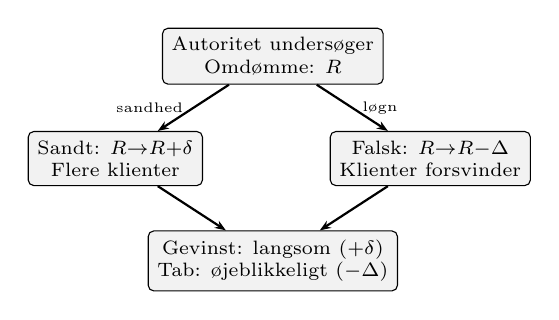
\begin{tikzpicture}[
    box/.style={draw, rounded corners=2pt, minimum width=2cm, minimum height=0.6cm, align=center, font=\scriptsize, fill=black!5},
    arr/.style={-{Stealth[length=4pt]}, thick}
]
\node[box] (exam) at (0,0) {Autoritet undersøger\\Omdømme: $R$};
\node[box] (true) at (-2,-1.3) {Sandt: $R{\to}R{+}\delta$\\Flere klienter};
\node[box] (false) at (2,-1.3) {Falsk: $R{\to}R{-}\Delta$\\Klienter forsvinder};
\node[box] (insight) at (0,-2.6) {Gevinst: langsom ($+\delta$)\\Tab: øjeblikkeligt ($-\Delta$)};

\draw[arr] (exam) -- node[left,font=\tiny] {sandhed} (true);
\draw[arr] (exam) -- node[right,font=\tiny] {løgn} (false);
\draw[arr] (true) -- (insight);
\draw[arr] (false) -- (insight);
\end{tikzpicture}
\caption{Omdømmeautoritet---asymmetriske incitamenter.}
\label{fig:authority}
\end{figure}

\subsection{Flerdimensionelt Omdømme}

Omdømme er ikke en skalar, men en vektor på tværs af flere dimensioner: finansiel pålidelighed, personlig integritet, faglig kompetence, borgerligt engagement og andre (Fig.~\ref{fig:reputation-radar}). Forskellige evalueringsudbydere projicerer denne vektor forskelligt afhængigt af kontekst---en långiver prioriterer finansiel pålidelighed, en arbejdsgiver faglig kompetence, en nabo borgerlig adfærd. Der findes ingen enkelt ``korrekt'' omdømmescore; kun perspektiver.

\begin{figure}[ht]
\centering
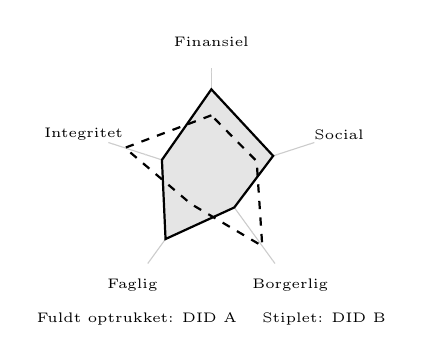
\begin{tikzpicture}[scale=0.55]
\foreach \a/\l in {90/Finansiel,162/Integritet,234/Faglig,306/Borgerlig,18/Social} {
  \draw[gray!40] (0,0) -- (\a:2.5);
  \node[font=\tiny, align=center] at (\a:3.1) {\l};
  \foreach \r in {0.8,1.6,2.4} {
    \fill[black!15] (\a:\r) circle (0.5pt);
  }
}
\draw[thick, fill=black!10] (90:2.0) -- (162:1.2) -- (234:1.8) -- (306:0.9) -- (18:1.5) -- cycle;
\draw[thick, dashed] (90:1.4) -- (162:2.1) -- (234:0.8) -- (306:2.0) -- (18:1.1) -- cycle;
\node[font=\tiny] at (0,-3.3) {Fuldt optrukket: DID A \quad Stiplet: DID B};
\end{tikzpicture}
\caption{Flerdimensionelle omdømmevektorer. Forskellige DID'er udviser forskellige profiler på tværs af dimensioner.}
\label{fig:reputation-radar}
\end{figure}

\subsection{Demokratiseret Risikovurdering}

RSN demokratiserer systematisk risikovurdering---en kapacitet, der i øjeblikket er koncentreret i finansielle institutioner, men anvendelig langt ud over bankvirksomhed. Industrielle konglomerater, der vurderer leverandørpålidelighed, forsikringsselskaber, der prissætter adfærdsrisiko, due diligence ved fusioner og opkøb, estimering af udstyrs levetid i produktion---overalt hvor modpartsrisiko kræver vurdering, tilvejebringer RSN et decentraliseret, markedsdrevet alternativ. Et marked af fortolkningstjenester oversætter rå flerdimensionelle omdømmedata til handlingsrettede sammendrag, hvilket gør modpartsevaluering tilgængelig for enhver deltager til marginalomkostning.

% ============================================================
% 7. CONSENSUS AND DISPUTE RESOLUTION
% ============================================================
\section{Konsensus og Tvistbilæggelse}

\subsection{Model for Decentraliseret Retfærdighed}

RSN omformulerer retfærdighed som et bilateralt forhandlingsproblem. Truslen om permanent, verificerbar omdømmeskade er et mere effektivt afskrækkelsesmiddel end retssager, som den skadelidte part ikke har råd til.

\subsection{Emergent Konsensus}

Hver deltager opretholder en personlig tilfredshedstærskel. Netværkets samlede konsensus opstår som det statistiske gennemsnit af tusindvis af bilaterale forhandlinger (Fig.~\ref{fig:consensus}). Et svar langt over konsensus (barbarisk) er dyrt at publicere. Et svar nær konsensus (forholdsmæssigt) er billigt. Konsensus er ikke en regel---det er et prissignal.

\begin{figure}[ht]
\centering
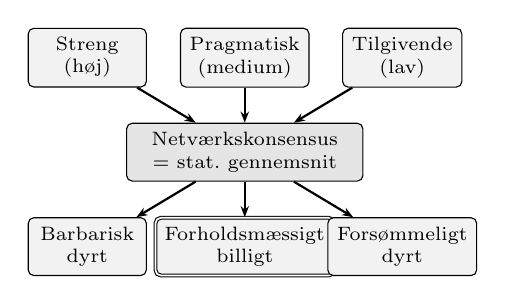
\begin{tikzpicture}[
    person/.style={draw, rounded corners=2pt, minimum width=1.5cm, minimum height=0.5cm, align=center, font=\scriptsize, fill=black!5},
    arr/.style={-{Stealth[length=4pt]}, thick}
]
\node[person] (a) at (-2,0) {Streng\\(høj)};
\node[person] (b) at (0,0) {Pragmatisk\\(medium)};
\node[person] (c) at (2,0) {Tilgivende\\(lav)};
\node[person, fill=black!10, minimum width=3cm] (cons) at (0,-1.2) {Netværkskonsensus\\= stat.\ gennemsnit};
\node[person] (exp) at (-2,-2.4) {Barbarisk\\dyrt};
\node[person, double] (prop) at (0,-2.4) {Forholdsmæssigt\\billigt};
\node[person] (neg) at (2,-2.4) {Forsømmeligt\\dyrt};

\draw[arr] (a) -- (cons);
\draw[arr] (b) -- (cons);
\draw[arr] (c) -- (cons);
\draw[arr] (cons) -- (exp);
\draw[arr] (cons) -- (prop);
\draw[arr] (cons) -- (neg);
\end{tikzpicture}
\caption{Emergent konsensus ud fra individuelle tilfredshedstærskler.}
\label{fig:consensus}
\end{figure}

\subsection{Kalibrering af Straf}

Hver DID-Indehaver erklærer offentligt reaktioner på specifikke kategorier af forseelser. Uforholdsmæssigt hårde eller milde erklæringer tiltrækker negative omdømmesignaler. Forholdsmæssige erklæringer accepteres uden friktion---et selvkalibrerende strafsystem.

Konsensuserklæringer er selv underlagt hykleridetektion: deklarativt at forpligte sig til en konsensusposition, mens man opfører sig inkonsekvent, udgør en omdømmemæssig forseelse, der er alvorligere end den underliggende afvigelse, da den demonstrerer forsætligt bedrag.

\subsection{Delegering}

Alle aktiviteter inden for en DID---med én undtagelse---kan delegeres til en anden DID. \textbf{Subjekt-rollen---den DID, hvis adfærd påstanden handler om---kan ikke delegeres; den er uigenkaldeligt bundet til den identitetsindehaver, som påstanden refererer til.} De øvrige aktive roller---Udsteder, Autoritet, Vidne, Verifikator---kan overføres til en udpeget delegat-DID, hvad enten det er til verifikation, indsendelse af påstande, deltagelse i konsensus eller tvistbilæggelse. Delegering kan til enhver tid tilbagekaldes. Dette muliggør specialisering (f.eks. professionelle verifikationstjenester), mens Indehaveren bevarer den endelige kontrol og ansvar. Delegering gælder på tværs af hele systemet og er afgørende for skalerbarhed.

\subsection{Fra Individuel Moral til Emergent Samfundskontrakt}

Hver DID's erklærede policy repræsenterer en formalisering af individuel moral: hvad Indehaveren anser for acceptabelt, hvordan de reagerer på specifik adfærd, hvad de kræver af modparter. Disse policyer er ikke pålagt af en systemdesigner---de vælges af hver deltager og udtrykkes i maskinlæsbar form.

Denne formalisering muliggør en tretrins-emergens. Først kodes individuel moral som \textbf{policy}---et sæt erklærede regler, tærskler og responsfunktioner, som DID'en forpligter sig til at følge. Dernæst producerer summen af alle policyer på tværs af netværket \textbf{emergent etik}---statistisk observerbare normer, som ingen enkelt deltager udformede, men som opstår ud af interaktionen mellem tusindvis af individuelle moralske positioner~\cite{durkheim1893}. For det tredje udgør denne emergente etik, udtrykt som fælles adfærdsnormer håndhævet gennem bilaterale prissignaler, en \textbf{målbar samfundskontrakt}---ikke en teoretisk konstruktion, som ingen underskrev~\cite{rawls1971}, men et empirisk observerbart sæt regler underbygget af faktisk adfærd.

Denne proces afspejler resultater fra moralfundamentsteori~\cite{haidt2012}: menneskelig moral er intuitiv, pluralistisk og kulturelt variabel. RSN kræver ikke moralsk konsensus som input; det producerer adfærdsmæssig konsensus som output. Den resulterende samfundskontrakt er ikke statisk---den udvikler sig, efterhånden som deltagere tilslutter sig, forlader og justerer deres policyer som reaktion på netværksfeedback. I modsætning til klassisk samfundskontraktteori er denne kontrakt tilbagekaldelig, observerbar og håndhævelig uden en suveræn.

% ============================================================
% 8. ECONOMIC MODEL
% ============================================================
\section{Økonomisk Model}

De foregående afsnit beskrev et værktøj---RSN's verifikationsmekanismer, omkostningsstruktur og emergente konsensus. Dette afsnit beskriver en metodologi for anvendelse af dette værktøj på finanspolitisk og forvaltningsmæssig overgang. Værktøjet er til almen brug; nedenstående metodologi er én mulig anvendelse.

\subsection{Incitamentsstruktur}

Omdømme som kapital skaber direkte incitamenter for hæderlig adfærd. Under normal drift opbygger deltagere naturligt omdømme gennem daglige transaktioner og opfyldte forpligtelser. Den primære udgift er på \emph{negative} påstande---registrering af skade forvoldt af andre. Denne asymmetri tilskynder til nyttig, pålidelig adfærd: at være hæderlig koster ikke ekstra, mens at være skadelig skaber et dokumenteret spor, som andre vil betale for at bevare. Hykleri---at erklære regler uden at følge dem---er den dyreste fejltilstand, da den demonstrerer forsætligt bedrag.

\subsection{Parallelt Finanspolitisk System}

Tre komponenter muliggør konkurrencepres: (1)~\textbf{Simpel Skat}---en enkelt proportional sats uden undtagelser, indledningsvis marginalt under den eksisterende effektive sats; (2)~\textbf{Elektronisk Registrering af Udgifter (ESR)}---en omvendt version af den tjekkiske EET-model, så borgere overvåger statens udgifter; (3)~\textbf{Borgerstyret Skatteallokering}---begyndende ved nogle få procent i det første år og efter et årti nående alt fra lave tocifrede tal til en fuld migration til et borgerstyret system, afhængigt af udbredelsestempoet. Det faktiske tempo afhænger af hastigheden, hvormed frimarkedsalternativer til statslige tjenester opstår, og af statens vilje til at samarbejde om overgangen; tidsfunktionen behøver ikke være lineær, og der er ingen grund til at fastsætte en øvre grænse for, hvor udbredelsen i sidste ende kan nå.

% ============================================================
% 9. MIGRATION PATH
% ============================================================
\section{Migrationsvej}

Migrationen forløber gennem tre faser (Fig.~\ref{fig:migration}): \textbf{Fase~1: Overlejring} (RSN som informationslag, staten er eneste udbyder), \textbf{Fase~2: Konkurrence} (RSN tilvejebringer funktionelle alternativer, brug af to systemer) og \textbf{Fase~3: Overgang} (RSN overgår statslige modstykker, frivillig migration). Overgangen er reversibel på ethvert stadie.

\begin{figure}[ht]
\centering
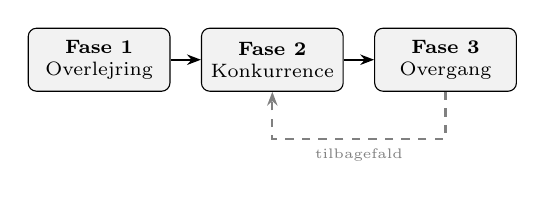
\begin{tikzpicture}[
    phase/.style={draw, rounded corners=3pt, minimum width=1.8cm, minimum height=0.8cm, align=center, font=\scriptsize, fill=black!5},
    arr/.style={-{Stealth[length=5pt]}, thick}
]
\node[phase] (p1) at (0,0) {\textbf{Fase 1}\\Overlejring};
\node[phase] (p2) at (2.2,0) {\textbf{Fase 2}\\Konkurrence};
\node[phase] (p3) at (4.4,0) {\textbf{Fase 3}\\Overgang};

\draw[arr] (p1) -- (p2);
\draw[arr] (p2) -- (p3);
\draw[arr, dashed, gray] (p3.south) -- ++(0,-0.6) -| node[below,font=\tiny,pos=0.25] {tilbagefald} (p2.south);
\end{tikzpicture}
\caption{Trefaset migration---reversibel på ethvert stadie.}
\label{fig:migration}
\end{figure}

Den primære pressmekanisme er finanspolitisk: når betingede skatteydere når et ``økonomisk betydeligt mindretal $X$''---en gruppe stor nok til, at undertrykkelse mod den forårsager ikke-triviel økonomisk skade, og civil ulydighed bliver en troværdig trussel---indtræder staten i forhandling. Til illustration bruger vi $X \approx 15\%$ af BNP, men den faktiske tærskel afhænger af den specifikke økonomi.

% ============================================================
% 10. SECURITY ANALYSIS
% ============================================================
\section{Sikkerhedsanalyse}

Vi betragter fem kategorier af modstandere: individuelle onde aktører, organiserede grupper, virksomhedsmodstandere, statslige modstandere og modstandere på protokolniveau.

\textbf{Sybil-modstandsdygtighed}~\cite{douceur2002}. At opbygge omdømme kræver vedvarende, verificerbar interaktion. Omkostningen ved et vellykket Sybil-angreb skalerer lineært med antallet af falske identiteter og kvadratisk med målomdømmets niveau. At drive flere DID'er parallelt er muligt, men dyrt af design---hver identitet skal uafhængigt akkumulere omdømme gennem ægte aktivitet. I frie samfund afskrækker denne omkostning tilfældigt misbrug; i diktaturer bliver parallelle DID'er et overlevelsesredskab, der muliggør opdelt modstand, underjordisk koordinering og sikrere navigering på det sorte marked.

\textbf{Forsvar mod hemmelig aftale.} Mønstre af gensidig godkendelse blandt lukkede grupper er detekterbare gennem analyse af den sociale graf. Omdømmeaggregeringsfunktioner nedvægter påstande fra tæt sammenklyngede kilder.

\textbf{Modstander på statsniveau.} Onion-routing, fravær af centraliseret infrastruktur og fordeling af Verifikator-rollen på tværs af deltagerbasen sikrer, at undertrykkelse kræver foranstaltninger, der er uforholdsmæssige i forhold til enhver fordel.

\textbf{Privatliv vs.\ ansvarlighed.} Pseudonymitet---en mellemvej mellem anonymitet og identitetsafsløring---giver DID'er mulighed for at akkumulere meningsfuldt omdømme uden at afsløre Indehaverens virkelige identitet.

% ============================================================
% 11. PRIVACY
% ============================================================
\section{Privatlivsbetragtninger}

RSN's privatlivsmodel er bygget på pseudonymitet. Indehaveren kontrollerer identitetsafsløring: minimal (rent pseudonym), selektiv (specifikke legitimationsoplysninger tilknyttet) eller fuld (juridisk identitet tilknyttet). Publicerede påstande er permanente---systemet understøtter kontekstuel korrektion, men ikke sletning. En Indehaver kan opgive en kompromitteret DID og starte forfra og derved fortabe akkumuleret omdømme.

% ============================================================
% 12. RELATED WORK
% ============================================================
\section{Beslægtet Arbejde}

W3C DID Core-specifikationen~\cite{did2022} og Ceramic Network~\cite{ceramic2023} tilvejebringer identitetsgrundlaget. EigenTrust~\cite{kamvar2003} demonstrerede distribueret omdømmeaggregering uden central autoritet. SBT'er~\cite{weyl2022} introducerede ikke-overførbare sociale tokens. RSN adskiller sig ved sin vægt på økonomisk omkostning som et kvalitetsfilter og sin mekanisme til prissætning af radikalisme.

DAO'er~\cite{buterin2014} og kvadratisk afstemning~\cite{buterin2019} demonstrerede gennemførligheden af decentraliseret forvaltning. RSN udleder konsensus fra bilaterale prisforhandlinger snarere end afstemning.

Forslaget bygger på anarko-kapitalistisk teori~\cite{rothbard1973,hoppe2001} for privat tjenesteudbud, men afviger på to afgørende punkter: det designer for ondskabsfuldhed og gengældende impulser snarere end at antage rationalitet, og det foreslår gradvis overgang snarere end revolution. Konceptet om emergente samfundskontrakter har forgængere i Hayeks teori om spontan orden~\cite{hayek1973}.

\textbf{Anarko-agorisme.} RSN deler betydelig fælles grund med agoristisk modøkonomi~\cite{konkin2006}---særligt vægten på at opbygge parallelle institutioner og frivillig udveksling. Agorisme har imidlertid en tendens til at antage rationel egeninteresse som en tilstrækkelig koordineringsmekanisme og mangler ofte en konkret migrationsvej fra eksisterende statsstrukturer. RSN indarbejder eksplicit ikke-rationelle adfærdstilbøjeligheder og tilvejebringer en finanspolitisk pressmekanisme for gradvis overgang.

\textbf{Meritokrati.} RSN kan repræsentere en første funktionel beskrivelse af, hvordan meritokrati~\cite{young1958} kan opstå som en systemisk egenskab snarere end et slogan. Traditionelle meritokratiske systemer fejler, fordi de kræver en central autoritet til at definere og håndhæve ``fortjeneste''. I RSN opstår fortjeneste ud fra bilaterale evalueringer: de, der leverer værdi, akkumulerer omdømme; ingen komité afgør, hvem der har fortjeneste.

\textbf{Ejendom som privilegium.} RSN afviger grundlæggende fra anarko-kapitalistiske og østrigsk-skoles behandlinger af ejendomsrettigheder som naturlige og absolutte. I RSN-rammen er ejendom et \emph{privilegium}---en social anerkendelse, der i ekstreme tilfælde kan trækkes tilbage af fællesskabet, når en deltager fundamentalt overtræder fælles normer (forræderi, nægtelse af at forsvare fællesskabet i eksistentiel krise, systematisk udnyttelse). Dette er ikke statsekspropriation, men en tilbagetrækning af social anerkendelse fra netværket af bilaterale relationer.

% ============================================================
% 13. LIMITATIONS
% ============================================================
\section{Diskussion og Begrænsninger}

\textbf{Kold start.} RSN's værdi afhænger af netværkseffekter; tidlige brugere står over for begrænset værdi, indtil deltagelsen når en tærskel. Selv fra tidlige stadier tjener DID-netværket dog som en nyttig supplerende informationskilde. Tidlig omdømmeevaluering og autoritetsvurdering forventes at udvikle sig gradvist med stigende raffinement.

\textbf{Anti-snylteri og adgangskontrol.} Mål-DID'er kan pålægge graduerede gebyrer og adgangsbegrænsninger på forespørgsler fra DID'er med lavt omdømme. Dette er ikke binært, men en kontinuerlig skala: jo mindre omdømme en forespørgende DID har, jo mindre information modtager den, jo længere venter den, og jo mere betaler den. Denne mekanisme tilskynder til ægte deltagelse frem for passivt forbrug.

\textbf{Ulighed i adgang.} Omkostningen ved at publicere påstande kan bortfiltrere legitime klager fra økonomisk dårligt stillede deltagere. Afbødning: enhver deltager tjener samtidig som potentiel verifikator (eller delegerer denne rolle) og optjener verifikationsgebyrer. Over en tilstrækkelig tidshorisont bør en ikke-radikal deltager nærme sig finansiel neutralitet---verifikationsindtægt der omtrent opvejer publiceringsomkostninger. Dette er en statistisk forventning, ikke en garanti.

\textbf{Omdømmeulighed.} Tidlige brugere akkumulerer fordele, der kan skabe barrierer for sent tilkomne. Omdømmeevaluering udføres imidlertid af tredjepartsudbydere, der kan vælge at afbøde first-mover-fordelen gennem deres aggregeringsalgoritmer. At være først med et godt omdømme er en legitim komparativ økonomisk fordel---og det er tilsigtet.

\textbf{Åbne spørgsmål.} Optimale omkostningsfunktioner, aggregeringsstandarder, protokolforvaltning og interaktion med AI-genererede syntetiske omdømmedata forbliver områder for fremtidigt arbejde.

Denne artikel hævder ikke, at RSN vil producere optimale resultater under alle omstændigheder. Den hævder, at RSN repræsenterer et \emph{gennemførligt} alternativ---teknisk implementerbart, økonomisk selvbærende og socialt foreneligt med menneskelige adfærdstilbøjeligheder, som de faktisk er.

% ============================================================
% 14. CONCLUSION
% ============================================================
\section{Konklusion}

Denne artikel har præsenteret Omdømmesocialt Netværk, en decentraliseret protokol, der muliggør pseudonym, verificerbar omdømmeudveksling. Princippet om Dyr Radikalisme sikrer, at bedrageriske påstande prissættes ud uden censur. Den foreslåede migrationsvej muliggør gradvis, reversibel overgang fra eksisterende institutioner. Designet indarbejder den menneskelige natur, som den er---herunder smålighed, ondskabsfuldhed og ønsket om gengældende tilfredsstillelse---snarere end at kræve ideologisk transformation. Resultatet er ikke utopi, men et system, hvor retfærdighed er tilgængelig, omdømme optjenes, og omkostningen ved forseelser bæres af den part, der forårsagede den.

% ============================================================
% REFERENCES
% ============================================================
\bibliography{references}

\end{document}
